\section{Cluster Analysis for Climatic Regions}

Cluster analysis is a powerful unsupervised machine learning technique used to identify natural groupings within data. In the context of climate science, cluster analysis helps uncover regions with similar climatic behavior, even when they may be geographically distant.

The idea is simple: group together climate observations that are more similar to each other than to those in other groups. This allows researchers and policymakers to:
\begin{itemize}
    \item Identify climate zones based on observed data (e.g., temperature, precipitation, humidity).
    \item Compare regional climate behaviors.
    \item Tailor climate adaptation strategies to similar zones.
\end{itemize}

\subsection*{How It Works}

Let’s say we have a dataset with climate measurements such as temperature, humidity, precipitation, and wind speed. Each row in our data represents a region or time-point, and our goal is to group these rows into “clusters” of similar climate patterns.

Key steps in the clustering process:
\begin{enumerate}
    \item \textbf{Feature Selection:} Choose the relevant variables (e.g., temperature, humidity).
    \item \textbf{Standardization:} Scale the variables so that each contributes equally to the clustering.
    \item \textbf{Choosing the Number of Clusters (K):} Decide how many climate groups to form using techniques like the elbow method.
    \item \textbf{Applying Clustering Algorithm:} Use algorithms like k-means to partition the data into K clusters.
    \item \textbf{Interpretation:} Analyze and visualize the clusters to understand regional patterns.
\end{enumerate}

\subsection*{Cluster Analysis for Climatic Patterns}

\textbf{Understanding the Goal}\\

Imagine you’re handed a huge table full of weather data with temperature, precipitation, humidity, and more from different regions or time periods. A natural question might arise: “Can we group these observations into meaningful climate categories?”

That’s where clustering helps. It automatically finds groups (called clusters) in your data that share similar features. Here, we want to find such clusters based on:
\begin{itemize}
    \item \texttt{Temp\_2m} – Temperature at 2 meters height
    \item \texttt{Precip} – Precipitation
\end{itemize}

\textbf{Step-by-Step Exploration}\\

\textbf{Step 1: Clean the Data} \\
Before we do any analysis, it’s important to make sure the data we’re using is complete. Missing values can interfere with calculations. So, we begin by removing any rows where \texttt{Temp\_2m} or \texttt{Precip} is missing.
\begin{verbatim}
climate_data_clean <- climate_data[complete.cases(climate_data$Temp_2m,
climate_data$Precip), ]
\end{verbatim}

\textbf{Step 2: Standardize the Data} \\
Temperature and precipitation are measured on different scales. Standardizing (scaling) makes sure each feature contributes equally to the clustering.
\begin{verbatim}
climate_scaled <- scale(climate_data_clean[, c("Temp_2m", "Precip")])
\end{verbatim}

\textbf{Step 3: Apply K-Means Clustering} \\
Now, we use a popular method called k-means clustering. We tell it to group the data into 3 clusters (this can be adjusted using the elbow method).
\begin{verbatim}
kmeans_result <- kmeans(climate_scaled, centers = 3, nstart = 10)
\end{verbatim}

Each observation is assigned a cluster number (1, 2, or 3), which we add back to the dataset:
\begin{verbatim}
climate_data_clean$Cluster <- as.factor(kmeans_result$cluster)
\end{verbatim}

\textbf{Step 4: Visualize the Clusters} \\
Let’s now “see” what those clusters look like. We plot temperature against precipitation, coloring each point by its cluster.
\begin{verbatim}
ggplot(climate_data_clean, aes(x = Temp_2m, y = Precip, color = Cluster)) +
  geom_point(size = 3) +
  labs(
    title = "Clustering of Climate Data (Temp_2m vs Precip)", 
       x = "Temperature (2m)", y = "Precipitation", color = "Cluster") +
  theme_minimal()
\end{verbatim}

\begin{figure}[h]
\centering
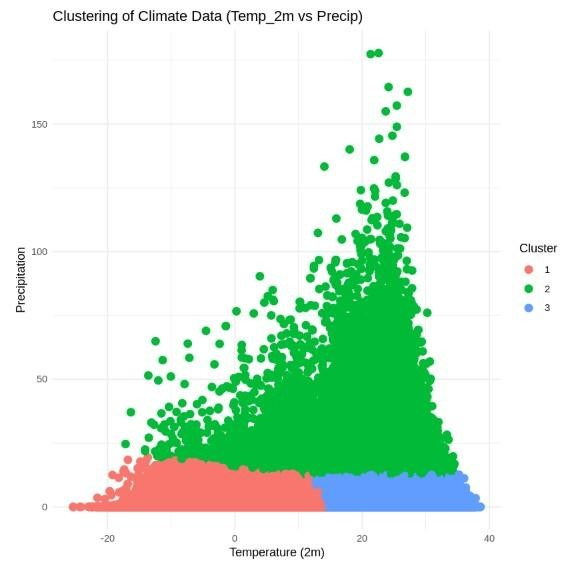
\includegraphics[width=0.5\textwidth]{figures/cluster.jpg}
\caption{Cluster Analysis for Climatic Patterns}
\end{figure}

Each color represents one cluster. The points in a cluster are close together, showing similar climate behavior.

\textbf{Why This Matters?}
\begin{itemize}
\item Clustering helps simplify large datasets into meaningful patterns. 
\item Each group can be analyzed separately to understand its unique climate profile. 
\item It’s useful for zoning, planning, and understanding environmental changes.
\end{itemize}

\textbf{Next Steps}\\

Now that we’ve performed basic clustering using k-means, we can explore:
\begin{itemize}
    \item Using more variables (e.g., humidity, pressure).
    \item Trying different clustering techniques (like hierarchical clustering).
    \item Mapping clusters onto geographical locations.
\end{itemize}
